\section{Lanczos正交化}
\label{sec:ls-lanczos}

第~\ref{sec:ls-arnoldi}节的Arnoldi正交化对一般方阵生成$\mathcal K_k(\bm A,\bm r_0)$的标准正交基，代价是每轮都要与全部旧基向量正交化。$\bm A$对称时，其中大部分系数自动为零。\term{Lanczos过程}（Lanczos process）就是Arnoldi正交化在对称矩阵上的简化：每轮只扣除两个方向，就生成同一组标准正交基，并把$\bm A$在子空间上的作用记录为一个对称三对角小矩阵。下面先推出三项递推，再写出计算过程，然后分析所得结果，最后说明它怎样用于求解方程；与Arnoldi正交化相同的论证只作引用。

\subsection{主要思想}

Lanczos过程的任务与Arnoldi正交化相同，只是矩阵对称：给定对称矩阵$\bm A\in\mathbb R^{d\times d}$、初始残差$\bm r_0\ne\bm 0$与步数$k$，生成标准正交向量$\bm v_1,\ldots,\bm v_k$，使前$j$个向量张成$\mathcal K_j(\bm A,\bm r_0)$，第一个向量取$\bm v_1=\bm r_0/\lVert\bm r_0\rVert_2$。

\paragraph{三项递推}
从第~\ref{sec:ls-arnoldi}节的系数出发。精确算术下，Arnoldi正交化在第$j$轮扣除的系数为
\[
 h_{i,j}=\bm v_i^\top\bm A\bm v_j\quad(i\le j),
\]
并且由列关系~\eqref{eq:ls-arnoldi-column}，每个$\bm A\bm v_i$都是$\bm v_1,\ldots,\bm v_{i+1}$的组合。$\bm A$对称时，
\[
 h_{i,j}=\bm v_i^\top\bm A\bm v_j=(\bm A\bm v_i)^\top\bm v_j .
\]
当$i+1<j$时，$\bm A\bm v_i$所含的$\bm v_1,\ldots,\bm v_{i+1}$都与$\bm v_j$正交，所以$h_{i,j}=0$；

当$i=j-1$时，$h_{j-1,j}=(\bm A\bm v_{j-1})^\top\bm v_j$恰是上一轮的归一化系数$h_{j,j-1}$。

于是第$j$轮只剩对角系数$h_{j,j}$与归一化系数$h_{j+1,j}$需要计算。记
\begin{equation}
 a_j=h_{j,j},\qquad \gamma_j=h_{j+1,j},
 \label{eq:ls-lanczos-coefficients}
\end{equation}
并约定$\bm v_0=\bm 0$、$\gamma_0=0$，列关系~\eqref{eq:ls-arnoldi-column}化为
\begin{equation}
 \bm A\bm v_j=\gamma_{j-1}\bm v_{j-1}+a_j\bm v_j+\gamma_j\bm v_{j+1},\qquad a_j=\bm v_j^\top\bm A\bm v_j ,
 \label{eq:ls-arnoldi-lanczos}
\end{equation}
这就是\term{Lanczos三项递推}（Lanczos recurrence）。计算新向量时只需用到紧邻的三个量$\bm A\bm v_j$、$\bm v_j$与$\bm v_{j-1}$，不必保存整组基。

图~\ref{fig:solver-lanczos-three-directions}把三项递推与三对角形状对应起来。固定第$j$列时，只需紧邻的三个基方向；其他位置的系数因对称性和正交性为零。

\begin{figure}[!htb]
  \centering
  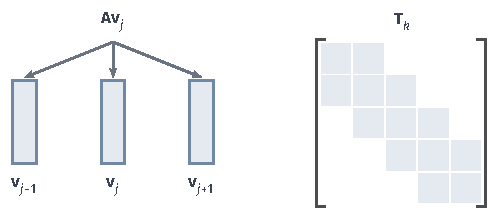
\includegraphics{figures/02-vectors-matrices-and-multivariate-calculus/03-linear-equations-and-optimization/tikz/learning-mechanisms/lanczos-three-directions.pdf}
  \caption{Lanczos过程在精确算术下的局部关系。左侧$\bm A\bm v_j$由$\bm v_{j-1},\bm v_j,\bm v_{j+1}$三个方向组成；右侧对称三对角矩阵$\bm T_k$只在主对角线和相邻两条对角线上可能非零。有限精度下可能需要重新正交化，图示不代表舍入后仍自动保持全局正交。}
  \label{fig:solver-lanczos-three-directions}
\end{figure}

\subsection{算法实现}

由三项递推~\eqref{eq:ls-arnoldi-lanczos}移项，每轮作一次矩阵乘向量，扣除两个方向，再把余项归一化。下面写出计算中用到的变量、它们怎样初始化、每轮怎样更新。下面用例~\ref{ex:ls-stationary-running-example}的以下数据逐步演示：
\[
 \bm A=\begin{bmatrix}4&1\\1&3\end{bmatrix},\qquad \bm b=\begin{bmatrix}1\\2\end{bmatrix}.
\]
取$\bm x_0=\bm 0$，于是$\bm r_0=\bm b$，步数取$k=2$。

\paragraph{变量}
\begin{itemize}
 \item $\bm v_{j-1},\bm v_j\in\mathbb R^d$：上一个与当前基向量，只保存这两个。
 \item $\bm w\in\mathbb R^d$：工作向量，先存$\bm A\bm v_j$，再在原处扣除两个方向，成为余项。
 \item $a_j$：第$j$个对角元。
 \item $\gamma_j$：第$j$个次对角元，也是$\bm v_{j+1}$的归一化系数；$\gamma_{j-1}$留到本轮扣除时使用。
 \item $j$：轮次。
\end{itemize}

\paragraph{初始化}
把上一个基向量初始化为零向量，$\gamma_0$初始化为零，第一个基向量初始化为初始残差的方向，轮次初始化为$1$：
\[
 \bm v_0=\bm 0,\qquad \gamma_0=0,\qquad \bm v_1=\frac{\bm r_0}{\lVert\bm r_0\rVert_2},\qquad j=1 .
\]
例中$\lVert\bm r_0\rVert_2=\sqrt5$，
\[
 \bm v_1=\frac1{\sqrt5}\begin{bmatrix}1\\2\end{bmatrix}.
\]

\paragraph{每轮更新}
在第$j$轮：
\begin{enumerate}
 \item \textbf{乘矩阵。}计算
 \[
  \bm w=\bm A\bm v_j .
 \]
 例中第一轮
 \[
   \bm w=\bm A\bm v_1=(6,7)^\top/\sqrt5 .
 \]

 \item \textbf{求对角元。}计算
 \[
  a_j=\bm v_j^\top\bm w .
 \]
 例中第一轮
 \[
   a_1=(1\cdot6+2\cdot7)/5=4 .
 \]

 \item \textbf{扣除两个方向。}计算
 \[
  \bm w\leftarrow\bm w-a_j\bm v_j-\gamma_{j-1}\bm v_{j-1} .
 \]
 例中第一轮$\gamma_0=0$，
 \[
  \bm w=\frac1{\sqrt5}\Bigl(\begin{bmatrix}6\\7\end{bmatrix}-4\begin{bmatrix}1\\2\end{bmatrix}\Bigr)=\frac1{\sqrt5}\begin{bmatrix}2\\-1\end{bmatrix}.
 \]

 \item \textbf{归一化。}计算
 \[
  \gamma_j=\lVert\bm w\rVert_2,\qquad \bm v_{j+1}=\frac{\bm w}{\gamma_j} .
 \]
 
 例中第一轮
 \[
  \gamma_1=1,\qquad \bm v_2=\frac1{\sqrt5}\begin{bmatrix}2\\-1\end{bmatrix}.
 \]
 然后令$j\leftarrow j+1$：$\bm v_j$成为下一轮的“上一个基向量”，$\bm v_{j+1}$成为“当前基向量”。

 例中第二轮先乘矩阵，得
 \[
  \bm w=\bm A\bm v_2=(7,-1)^\top/\sqrt5 ,
 \]
 再求对角元，
 \[
  a_2=\frac{14+1}{5}=3 .
 \]
 扣除$3\bm v_2$与$\gamma_1\bm v_1$后
 \[
  \bm w=\frac1{\sqrt5}\Bigl(\begin{bmatrix}7\\-1\end{bmatrix}-3\begin{bmatrix}2\\-1\end{bmatrix}-\begin{bmatrix}1\\2\end{bmatrix}\Bigr)=\bm 0 ,
 \]
 于是$\gamma_2=0$。

 \item \textbf{停止。}当$\gamma_j=0$（实际中低于按输入尺度取定的阈值）时，$\bm A\bm v_j$已落在现有空间中，Krylov子空间不再扩张，不作归一化，退出迭代；否则做满$k$轮后退出。例中第二轮$\gamma_2=0$，二维空间已经用尽，退出迭代。
\end{enumerate}
第1—4步合起来就是
\begin{equation}
 \begin{aligned}
 \bm w&=\bm A\bm v_j, & a_j&=\bm v_j^\top\bm w,\\
 \hat{\bm w}&=\bm w-a_j\bm v_j-\gamma_{j-1}\bm v_{j-1},\\
 \gamma_j&=\lVert\hat{\bm w}\rVert_2, & \bm v_{j+1}&=\hat{\bm w}/\gamma_j .
 \end{aligned}
 \label{eq:ls-lanczos-step}
\end{equation}
实际计算中也常先扣除$\gamma_{j-1}\bm v_{j-1}$，再用扣除后的向量求$a_j$：精确算术下结果相同，这与修正Gram--Schmidt的做法一致，有限精度下正交性略好。

最终得到标准正交基$\bm v_1,\bm v_2$与各轮系数组成的三对角矩阵。例中
\[
 \bm V_2=\frac1{\sqrt5}\begin{bmatrix}1&2\\2&-1\end{bmatrix},\qquad
 \bm T_2=\begin{bmatrix}a_1&\gamma_1\\\gamma_1&a_2\end{bmatrix}=\begin{bmatrix}4&1\\1&3\end{bmatrix},
\]
它们满足
\[
 \bm A\bm V_2=\bm V_2\bm T_2 .
\]
逐列核对：
\[
 \begin{gathered}
 4(1,2)^\top+(2,-1)^\top=(6,7)^\top,\\
 (1,2)^\top+3(2,-1)^\top=(7,-1)^\top ,
 \end{gathered}
\]
两边同除以$\sqrt5$即是$\bm A\bm v_1$与$\bm A\bm v_2$。

结果与第~\ref{sec:ls-arnoldi}节对同一矩阵算出的$\bm H_2$相同，但这里每轮只扣除了两个方向。

\subsection{算法分析}

\paragraph{基矩阵与投影矩阵}
与第~\ref{sec:ls-arnoldi}节一样，把各步的基并排成瘦长矩阵$\bm V_k=[\bm v_1,\ldots,\bm v_k]\in\mathbb R^{d\times k}$，它的列张成$\mathcal K_k$。把$j=1,\ldots,k$的递推式~\eqref{eq:ls-arnoldi-lanczos}按列并排写出，得到矩阵形式
\begin{equation}
 \bm A\bm V_k=\bm V_k\bm T_k+\gamma_k\bm v_{k+1}\bm e_k^\top=\bm V_{k+1}\overline{\bm T}_k ,
 \label{eq:ls-arnoldi-tridiagonal}
\end{equation}
其中
\begin{equation}
 \bm T_k=\begin{bmatrix}
 a_1&\gamma_1&&\\
 \gamma_1&a_2&\ddots&\\
 &\ddots&\ddots&\gamma_{k-1}\\
 &&\gamma_{k-1}&a_k
 \end{bmatrix},
 \label{eq:ls-lanczos-tridiagonal-matrix}
\end{equation}
$\overline{\bm T}_k$是在$\bm T_k$下方添一行$\gamma_k\bm e_k^\top$所得的$(k+1)\times k$矩阵。

左乘$\bm V_k^\top$，并用$\bm V_k^\top\bm V_k=\bm I$与$\bm V_k^\top\bm v_{k+1}=\bm 0$，得
\begin{equation}
 \bm T_k=\bm V_k^\top\bm A\bm V_k .
 \label{eq:ls-lanczos-projection}
\end{equation}
这正是Arnoldi关系~\eqref{eq:ls-arnoldi-relation}在对称情形下的形式：
\[
  \overline{\bm H}_k=\overline{\bm T}_k,\qquad \bm H_k=\bm T_k .
\]

$\bm T_k$同样是$\bm A$在$\mathcal K_k$上的投影，即子空间中向量的像在子空间中的坐标由$\bm T_k$给出；不同的是，它不仅是上Hessenberg矩阵，而且对称，因而是三对角的。

$d$维对称矩阵在子空间上的作用，就这样被压缩成一个$k$阶对称三对角矩阵，只需$2k-1$个数$a_1,\ldots,a_k$与$\gamma_1,\ldots,\gamma_{k-1}$记录。

\paragraph{正确性}
推导三项递推时用到了“此前各步的基已经标准正交”，这是由完整扣除保证的；只扣除两项时需要重新确认。下面的定理用归纳法证明这一点，并给出终止的情形。

\begin{theorem}[Lanczos关系]
\label{thm:ls-arnoldi-lanczos}
设$\bm A$对称，$\bm r_0\ne\bm 0$，在精确算术下按式~\eqref{eq:ls-lanczos-step}执行$k$轮，且$\gamma_1,\ldots,\gamma_{k-1}$均非零。若$\gamma_k\ne0$，则$\bm v_1,\ldots,\bm v_{k+1}$标准正交，$\bm v_1,\ldots,\bm v_j$张成$\mathcal K_j$（$j\le k+1$），关系~\eqref{eq:ls-arnoldi-tridiagonal}成立，并且$\bm T_k=\bm V_k^\top\bm A\bm V_k$。若$\gamma_k=0$，则$\bm v_1,\ldots,\bm v_k$标准正交，$\bm A\bm V_k=\bm V_k\bm T_k$，$\mathcal K_k$在$\bm A$下不变；$\bm A$非奇异时精确解$\bm x_\star$属于$\bm x_0+\mathcal K_k$。
\end{theorem}

\begin{proof}
依次证明正交性、张成关系与矩阵关系，最后处理子空间不再扩张的情形。

\emph{正交性。}对$j$归纳，设$\bm v_1,\ldots,\bm v_j$标准正交，且对$i<j$式~\eqref{eq:ls-arnoldi-lanczos}成立。只需证明扣除后的$\hat{\bm w}=\bm A\bm v_j-a_j\bm v_j-\gamma_{j-1}\bm v_{j-1}$与$\bm v_1,\ldots,\bm v_j$都正交。对$i=j$，由$a_j=\bm v_j^\top\bm A\bm v_j$，$\bm v_j^\top\hat{\bm w}=0$。对$i<j$，由对称性$\bm v_i^\top\bm A\bm v_j=(\bm A\bm v_i)^\top\bm v_j$，而$\bm A\bm v_i=\gamma_{i-1}\bm v_{i-1}+a_i\bm v_i+\gamma_i\bm v_{i+1}$，所以
\[
 \bm v_i^\top\bm A\bm v_j=\gamma_i\,\bm v_{i+1}^\top\bm v_j=
 \begin{cases}\gamma_{j-1},&i=j-1,\\0,&i<j-1.\end{cases}
\]
再由$\bm v_i^\top\bm v_{j-1}$与$\bm v_i^\top\bm v_j$的取值，$i=j-1$时$\bm v_{j-1}^\top\hat{\bm w}=\gamma_{j-1}-\gamma_{j-1}=0$，$i<j-1$时三项都为零。$\gamma_j\ne0$时归一化得到单位向量$\bm v_{j+1}$，与前$j$个正交。

\emph{张成与矩阵关系。}$\bm v_1\in\mathcal K_1$；若$\bm v_{j-1},\bm v_j\in\mathcal K_j$，则
\[
 \bm v_{j+1}\in\operatorname{span}\{\bm A\bm v_j,\bm v_j,\bm v_{j-1}\}\subseteq\mathcal K_{j+1},
\]
$j+1$个标准正交向量落在维数不超过$j+1$的$\mathcal K_{j+1}$中，因而张成它。由式~\eqref{eq:ls-lanczos-step}，$\gamma_j\bm v_{j+1}$就是扣除后的余项，把扣除的两项加回即得列关系~\eqref{eq:ls-arnoldi-lanczos}，并排写出即是式~\eqref{eq:ls-arnoldi-tridiagonal}。左乘$\bm V_k^\top$，并用$\bm V_k^\top\bm V_k=\bm I$与$\bm V_k^\top\bm v_{k+1}=\bm 0$，得$\bm T_k=\bm V_k^\top\bm A\bm V_k$。

\emph{不再扩张的情形。}若$\gamma_k=0$，第$k$列成为$\bm A\bm v_k=\gamma_{k-1}\bm v_{k-1}+a_k\bm v_k$，于是$\bm A\bm V_k=\bm V_k\bm T_k$，$\bm A\mathcal K_k\subseteq\mathcal K_k$。$\bm A$非奇异时它在有限维空间$\mathcal K_k$上是单射，因而也是满射；$\bm r_0\in\mathcal K_k$，故有$\bm z\in\mathcal K_k$使$\bm A\bm z=\bm r_0$，$\bm x_\star=\bm x_0+\bm z$。
\end{proof}

定理表明，精确算术下只扣除两项与扣除全部已有分量结果相同：被省略的系数$\bm v_i^\top\bm A\bm v_j$（$i<j-1$）本来就是零。第~\ref{sec:ls-arnoldi}节对一般方阵扣除全部已有分量，得到上Hessenberg小矩阵；$\bm A$对称时它退化为这里的$\bm T_k$，两种过程给出相同的基与系数，贯穿例上两节的数值也完全一致。$\mathcal K_k$的维数不超过$d$，所以至多$d$轮出现$\gamma_k=0$。

\paragraph{数值敏感度}
有限精度下，正交性依赖的相消只近似成立。三项递推只对最近两个方向扣除，舍入引入的旧方向分量不会被去掉，并且会随迭代放大，基的正交性损失比第~\ref{sec:ls-arnoldi}节的完整正交化明显；典型的表现是$\bm T_k$的特征值中出现$\bm A$同一特征值的多个近似副本。保存全部基并再正交化可以补救，但这就失去了固定存储的优点；不保存基时，调用它的求解器只能靠真实残差复核控制结果。

\paragraph{计算代价}
每轮一次$\bm A$乘向量，此外只有两次内积（其一用于求$\gamma_j$）、两次向量更新和一次缩放，约$9d$次浮点运算；除矩阵外保存$\bm v_{j-1},\bm v_j,\bm w$三个向量，存储不随轮数增长。与Arnoldi正交化$k$轮约$2dk^2$次运算、$(k+1)d$个数的存储相比，这是利用对称性得到的主要收益。本过程只负责生成候选空间，收敛快慢由调用它的求解器在子空间中采用的选解准则决定。

\subsection{应用}
\label{sec:ls-lanczos-application}

用法与第~\ref{sec:ls-arnoldi-application}节相同：把近似写成$\bm x_k=\bm x_0+\bm V_k\bm y$，$\bm y\in\mathbb R^k$是子空间中的坐标，再按某个准则确定$\bm y$。

按Galerkin条件，$\bm V_k^\top(\bm r_0-\bm A\bm V_k\bm y)=\bm0$，由$\bm r_0=\lVert\bm r_0\rVert_2\bm v_1$与$\bm T_k=\bm V_k^\top\bm A\bm V_k$，得到$k$阶三对角方程组
\begin{equation}
 \bm T_k\bm y=\lVert\bm r_0\rVert_2\,\bm e_1 .
 \label{eq:ls-lanczos-projected-system}
\end{equation}
它只有$k\times k$大小，又是三对角的，用第~\ref{sec:ls-lu}节的消元约$O(k)$次运算即可解出；解出坐标$\bm y$后，再用$\bm V_k$还原，就得到原空间中的近似解$\bm x_k$。

这就是后面两种对称矩阵求解器的共同骨架。对称正定时，$\bm T_k$也对称正定，方程~\eqref{eq:ls-lanczos-projected-system}总有唯一解，所得近似就是CG的迭代值（第~\ref{sec:ls-conjugate-gradient}节）；CG还利用$\bm T_k$的分解随步数延伸的结构，把求解与还原合并为短递推，连基$\bm V_k$也不必保存。

对称不定时，$\bm T_k$可能奇异，MINRES（第~\ref{sec:ls-minres}节）改用$(k+1)\times k$的$\overline{\bm T}_k$，在子空间中求残差最小的坐标：
\begin{equation}
 \min_{\bm y}\bigl\lVert\lVert\bm r_0\rVert_2\bm e_1-\overline{\bm T}_k\bm y\bigr\rVert_2 .
 \label{eq:ls-lanczos-minimal-residual-problem}
\end{equation}

两者的子空间、基和三对角矩阵都来自同一个Lanczos过程，区别只在于用哪一种准则确定坐标$\bm y$。
